\section{TCP/IP: Vazba mezi RM ISO/OSI a TCP/IP. Filozofie vzájemného propojování sítí. Souběh aplikací a zapouzdřování přenášených dat.}

\subsection{Vazba mezi RM ISO/OSI a TCP/IP}

Při vytváření tvůrci měli rozdílné přístupy.
V modelu ISO/OSI je důraz na vlastnosti sítě (spojovaný a spolehlivý charakter sítě) s tím že připojované hostitelské PC budou mít jednoduchou úlohu.
Ve výsledku se každá vrstva tohoto modelu snaží zajišťovat spolehlivost sama.
V modelu TCP/IP tvůrci vycházeli, že spolehlivost bude zajištěna koncovými účastníky.
Tím síť neztrácí kapacitu na zajištění spolehlivosti, tak že funguje na principu best-effort.
V TCP/IP se předpokládá jednoduchá síť s chytrými počítači.

\subsection{Vrstvy TCP/IP}

\begin{figure}[!h]
    \centering
    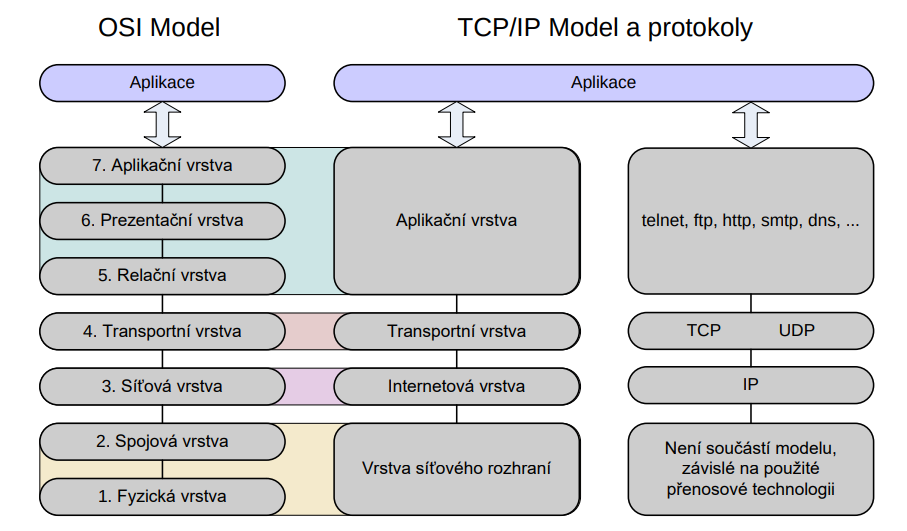
\includegraphics[width=0.9\textwidth]{obrazky/010.png}
\end{figure}

\textbf{Vrstva síťového rozhraní}\,--\,se stará o vše spojené s ovládáním konkrétní přenosové cesty (vysílání a příjem datových paketů).
Není specifikována a záleží na přenosové technologii.

\textbf{Internetová vrstva}\,--\,je realizovaná protokolem IP.
Má za cíl aby se jednotlivé pakety dostali od odesílatele ke koncovému příjemci.
Tento přenos probíhá přes mezilehlé směrovače.
Přenos je zajišťován datagramovou službou.

\textbf{Transportní vrstva}\,--\,je nejčasťeji realizována pomocí protokolu TCP. Má za úkol zajistit přenos mezi dvěma koncovými účastníky (nejčastěji 2 aplikační programy).
Dle požadavků a nároků těchto aplikačních programů transportní vrstva reguluje tok dat, zajišťuje spolehlivost přenosu a může měnit nespojovaný charakter přenosu na spojovaný.
Dále vrstva může využívat UDP protokolu pokud aplikace nepotřebují spolehlivost.
Vrstva může také využít SCTP protokol.

\textbf{Aplikační vrstva}\,--\,obsahuje jednotlivé aplikační programy, které komunikují přímo s transportní vrstvou na rozdíl od ISO/OSI.
Prezentační a relační vrstvy si aplikace musí implementovat sami.
Pokud tyto vrstvy aplikace nepotřebuje tak je nemusí implementovat a tím snížit režii při přenosu.

\subsection{Filozofie vzájemného propojování sítí}

Model TCP/IP se snaží o co nejuniverzálnější propojení sítí různých typů (lokální až celosvětové sítě).
Má při tom za cíl umožnit každému počítači komunikovat s každým počítačem bez ohledu na existenci přímého spojení nebo různých sítí.
Aplikace/uživatelé se na celou strukturu dívají pouze jako jednu velkou síť.
Na obrázku je komunikace mezi dvěma zařízeními přes síť.
Plná čára značí reálný průchod dat a přerušovaná čára značí virtuální spoje.

\begin{figure}[!h]
    \centering
    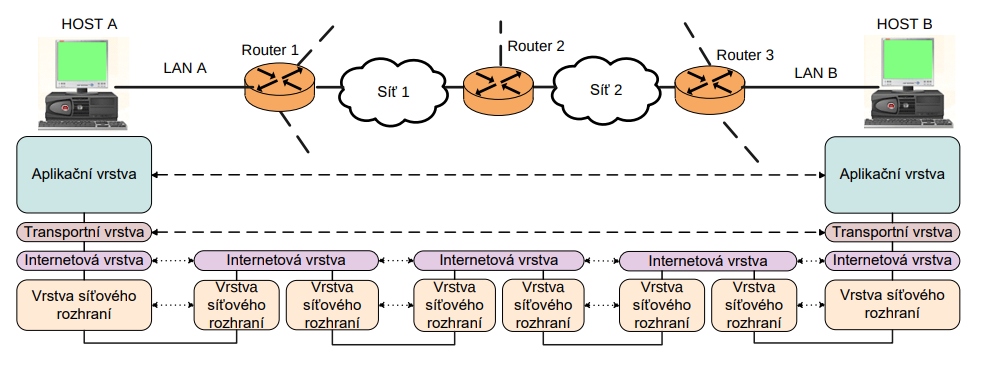
\includegraphics[width=0.75\textwidth]{obrazky/011.png}
\end{figure}

\subsection{Souběh aplikací a zapouzdřování přenášených dat}

\begin{figure}[!h]
    \centering
    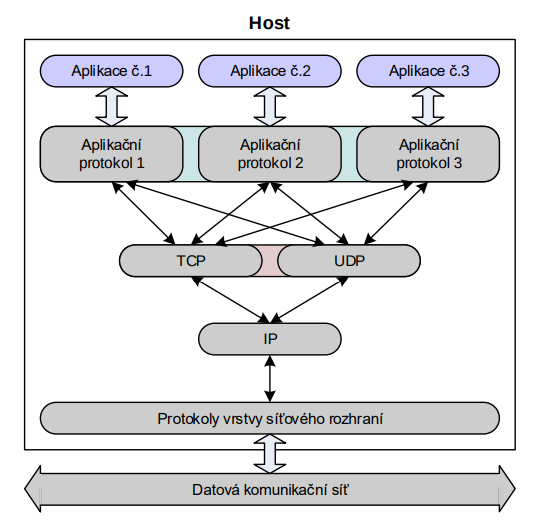
\includegraphics[width=0.45\textwidth]{obrazky/012.png}
\end{figure}

Na obrázku lze vidět souběh tří aplikací, kdy každá z těchto aplikací využívá jiný aplikační protokol (HTTP, FTP, POP, DNS, DHCP atd.).
Aplikace umí zformulovat uživatelské požadavky do zprávy, kterou druhá strana bude umět zpracovat.
Tato jednotka/zpráva se nazývá PDU (Protocol Data Unit).
Skládá se ze záhlaví APDU a dat.
PDU je dále předávána nižším vrstvám, které přidávají vlastní záhlaví a případně i zápatí.
Tomuto postupnému přidávání záhlaví se říká zapouzdřování.
Příklad obecného zapouzdření lze vidět na dalším obrázku.

\begin{figure}[!h]
    \centering
    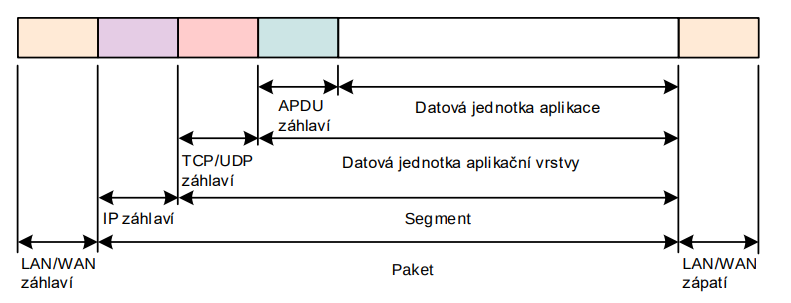
\includegraphics[width=0.6\textwidth]{obrazky/013.png}
\end{figure}


\clearpage
\section{Úloha IPv4 (Internet Protocol verze 4) vrstvy. IPv4 adresy. IPv4 datagram. IP tunelování. Protokol ICMPv4 (Internet Control Message Protocol verze 4).}

V modelu TCP/IP je IPv4 protokol využit na úrovni internetové vrstvy.
Zajišťuje potřebné směrování mezi dílčími sítěmi.
Musí pracovat s odlišnými adresami, různou maximální velikostí přenášených paketů atd.

\subsection{IPv4}

IPv4 adresa má délku 32 bitů.
Počet všech adres je označován jako \textbf{adresní prostor} s~velikostí $2^{32}$, tj. zhruba čtyři miliardy adres.
IPv4 adresy se zapisují jako čtyři čísla v~rozsahu $[0, 255]$ oddělena tečkou, např. \texttt{147.229.71.29}.

\textbf{Maska sítě} rozděluje IP adresu na~adresu sítě a~stanice.
Jde o~nepřerušenou řadu bitů zleva, která je reprezentována číslem $[1, 32]$ reprezentujícím počet bitů masky.
Adresa \texttt{147.229.71.29/24} znamená síť \texttt{147.229.71.0}, stanici \texttt{0.0.0.29} a~masku \texttt{255.255.255.0}: \texttt{11111111 11111111 11111111 00000000}.
Číslo za~lomítkem se označuje jako délka prefixu: prefix \texttt{/18} odpovídá masce \texttt{255.255.192.0}.

V~síti je první adresa rezervovaná pro~síť samotnou a~poslední adresa pro~všesměrové vysílání (pakety jsou doručovány všem v~síti); ostatní adresy mohou být přiřazeny stanicím.

Historicky se adresní prostor IPv4 rozděloval pomocí tříd. V~devadesátých letech se přešlo k~beztřídnímu adresování, což umožnilo prostor rozdělit efektivněji.

\subsection{IPv4 datagram}

\begin{figure}[!h]
    \centering
    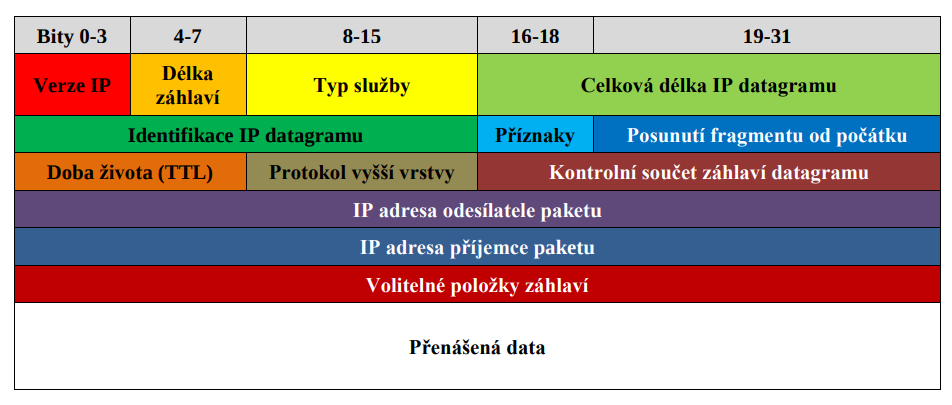
\includegraphics[width=0.8\textwidth]{obrazky/020.png}
\end{figure}

\subsection{IP tunelování}

Princip tunelování je zapouzdření původního paketu a~přidání nového záhlaví.
Záhlaví se liší tím, že má jinou cílovou a~zdrojovou IP adresu.

Typy tunelování:
\begin{itemize}[noitemsep]
    \item IP tunelování je vhodné pokud se přechází mezi verzemi IP protokolu (IPv4 a~IPv6). Při~přechodu mezi verzemi se přidá nové záhlaví před to původní.
    \item Tunelovaní spolu s~IPsec protokolem (celý packet je šifrován pomocí IPsec a~k~tomuto zašifrovanému paketu se přidá nové IP záhlaví).
\end{itemize}

\begin{figure}[!h]
    \centering
    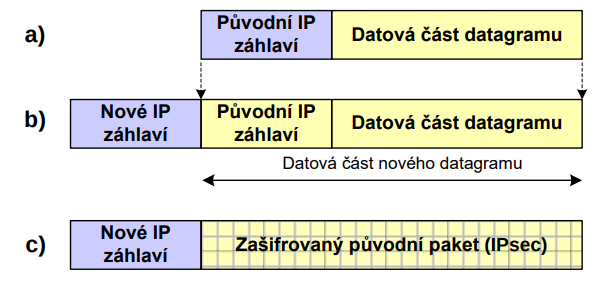
\includegraphics[width=0.6\textwidth]{obrazky/021.png}
\end{figure}


\subsection{ICMPv4}

Protokol ICMP je servisní protokol (nepřenáší žádná uživatelská data). Slouží k~testování konektivity, umožňuje signalizaci mimořádných událostí.

\begin{table}[ht]
	\centering
	\caption{Vybrané typy ICMP zpráv}
	\begin{tabular}{|l|c|l|}
		\hline
		kategorie    & typ & zpráva \\\hline\hline
		hlášení chyb & 3   & \emph{Destination unreachable} \\
		             & 4   & \emph{Source quench} (snížení rychlosti odesílání) \\
		             & 5   & \emph{Redirection} \\
		             & 11  & \emph{Time exceeded} \\
		             & 12  & \emph{Parameter problem} \\
		\hline
		dotazování   & 8   & \emph{Echo request} \\
		             & 0   & \emph{Echo reply} \\
		             & 13  & \emph{Timestamp request} \\
		             & 14  & \emph{Timestamp reply} \\
		\hline
	\end{tabular}
\end{table}



\clearpage
\section{Protokoly transportní vrstvy a jejich srovnání: UDP (User Datagram Protocol), Protokol TCP (Transmission Control Protocol), SCTP (Stream Control Transmission Protocol), protokol QUIC.}

\subsection{UDP user datagram protocol}

UDP je jednoduchý transportní protokol, který umožnuje nespojovaný a~nespolehlivý přenos dat (best effort). Přenášeným jednotkám se říká datagramy. Nepotvrzuje doručení musí být řešeno na~aplikační vrstvě. Oproti síťové umí UDP provádět přenos mezi konkrétními procesy. Má minimální režii přenosu a~zpoždění. Je vhodný na~přenos krátkých zpráv u~kterých není potřeba bezztrátovost.

\begin{figure}[!h]
    \centering
    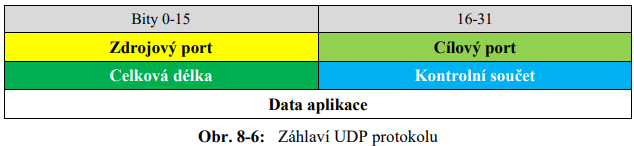
\includegraphics[width=0.7\textwidth]{obrazky/030.png}
\end{figure}

Zdrojový port určuje port na~straně odesílatele, cílový port na~straně příjemce, celková délka určuje velikost datagramu v~bytech a~kontrolní součet slouží k~základní detekci chyb.

Služby UDP:
\begin{itemize}[noitemsep]
    \item Komunikace proces--proces (komunikace socketových adres).
    \item Přenos dat bez spojení, každý datagram je přenášen samostatně (před komunikací není navozováno spojení).
    \item Žádné řízení toku dat, řízení proti zahlcení či řízení chybových stavů.
    \item Zapouzdřování a~odpouzdřování dat (pokud není detekována chyba).
    \item Frontování, multiplxování a~demultiplexování (fronty jsou vytvářeny dle portů) a~na těchto frontách lze provádět multiplexování a~demultiplexování.
\end{itemize}

Využití ve~službách dotaz-odpověď (DNS) nebo ve~VoIP službách.

\subsection{TCP Transmission Control Protocol}

TCP umožňuje spojovaný a~spolehlivý přenos dat. Přenášeným jednotkám se říká segmenty. Tyto segmenty jsou číslované. Číslovaní odesílaných a~potvrzovaných bytů (odeslané byty jedné strany, odeslané byty druhé strany, byty potvrzované jednou stanou a~byty potvrzované druhou stranou). Umožňuje řízení toku dat, chybových stavů a~stavů zahlcení. Má velkou režii přenosu.

\begin{figure}[!h]
    \centering
    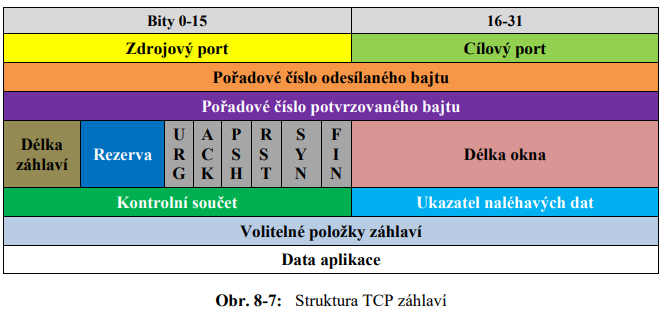
\includegraphics[width=0.7\textwidth]{obrazky/031.png}
\end{figure}

Pořadové číslo odesílaného bytu (SEQ, pořadové číslo prvního z~odeslaných bytů segmentu), pořadové číslo potvrzovacího bytu (ACK) hodnota dalšího očekávaného bytu, délka záhlaví (musí být uvedeno kvůli volitelným položkám záhlaví, které mají 0-40 bytů), příznakové bity (když jsou nastaveny na~1 jsou aktivní), délka okna (maximální počet odeslaných bytů aniž by bylo potřeba potvrzení přijímače), kontrolní součet (podobný UDP), ukazatel naléhavých dat (jen pokud URG je 1) a~volitelné položky záhlaví (nejsou povinná).

\vspace{1.5cm} % p5esunuto na dal39 str8nku aby v půlce seznamu nebyl obrázek
Příznakové bity:
\begin{itemize}[noitemsep]
    \item URG urgentní data
    \item ACK indikuje platnost pole potvrzovacího bytu
    \item PSH data mají být předána po~přijetí hned aplikaci (push)
    \item RST odmítnutí spojení
    \item SYN navazování spojení
    \item FIN ukončení spojení
\end{itemize}

Služby TCP:
\begin{itemize}[noitemsep]
    \item Komunikace proces--proces (komunikace socketových adres).
    \item Přenos toku dat (vytváří dojem propojení komunikujících procesů okruhem).
    \item Plně duplexní přenos dat (komunikace oběma směry zároveň).
    \item Multiplexování a~demultiplexování (stejné jako UDP).
    \item Spojovaně orientovaná služba (musí být prvně navázáno spojení a~na konci ukončeno).
    \item Spolehlivý přenos dat (využití potvrzovacích mechanizmů).
\end{itemize}

\begin{figure}[!h]
    \centering
    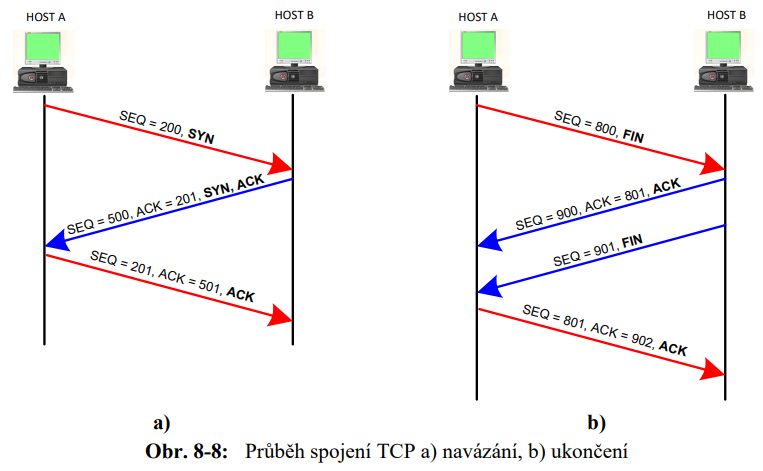
\includegraphics[width=0.7\textwidth]{obrazky/032.png}
\end{figure}

Navázání probíhá pomocí 3-cestného handshaku a~ukončení pomocí 4-cestného handshaku (existuje 3-cestná varianta na~obrázku kde ACK a~FIN jsou sloučeny do jedné zprávy).

Záhlaví TCP obsahuje délku okna sloužící k~nastavení přenosu maxima bytů bez potvrzení. Jelikož je spojení plně duplexní tak jsou okna vždy dvě a~nemusí mít stejnou velikost. Tento mechanismus se nazývá technika posuvného okna.

Využití na~službách HTTP, FTP, SMTP a~v dalších službách kde je potřeba spolehlivého přenosu.

\subsection{SCTP Stream Control Transmission Protocol}

Primární cílem bylo umožnit multimediální komunikaci s více IP adresami přiřazenými koncovým bodům komunikace.
Aktuálně je SCTP využívan například v mobilních 4G sítích.
SCPT je podobné protokolu TCP tím že je spojově orientovaný a poskytuje spolehlivý přenosový prostředek.
Z protokolu UDP využívá zachování hranic jednotlivých zpráv předávaných aplikační vrstvě.
Neboli pokud aplikace odešle zprávu o určité velikosti, je druhé zprávě předána stejná zpráva o stejné velikosti a to v jednom kroku.
U TCP může dojít k čekání na další zprávu při odesílání.

Unikátní funkcí SCTP je je využívání udržovacích zpráv označovaných jako \textit{Heartbeat/Keep-alive}.
Neslouží pro přenos dat ale pouze k zjišťování dostupnosti protistran a udržování jaká je hodnota Round Trip Time (RTT).
Dále umožňuje SCTP možnost specifikace délky života zprávy (Message Time-to-Live), jak dlouho má zpráva význam.
Pokud se nepodaří zprávu doručit v tomto časovém okně, odesílatel ji může zahodit.

\subsubsection{Multihoming a multistreaming}
Multihoming umožňuje přiřadit koncovému bodu při navazování spojení přiřadit více IP adres.
Jedna adresa je primární a druhá pak záložní.

Multistreaming umožňuje jedním transportním spojením přenášet více toků dat, které na sobě nemají být zcela závislé.
Dále je také částečně používán k zamezení stavu, kdy je komunikace blokována chybou či problémem na začátku přenosu určitého bloku dat.

\subsubsection{Struktura paketu}

\begin{figure}[!h]
    \centering
    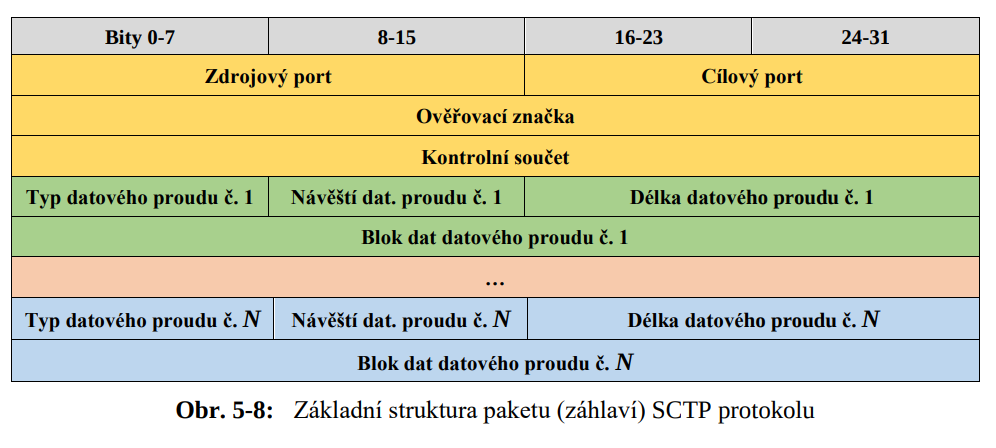
\includegraphics[width=0.7\textwidth]{obrazky/033.png}
\end{figure}

\begin{itemize}[noitemsep]
    \item Zdrojový a cílový port -- stejný jako u TCP a UDP
    \item Ověřovací značka -- ověření pravosti odesílatele paket
    \item Kontrolní součet -- využívá CRC32c algoritmus
    \item Typ datového proudu -- Definice co je přenášeno (DATA, INIT, INIT ACK, HEARTBEAT, \dots)
    \item Návěští datového proudu -- dle typu datové části, nemusí být využito
    \item Délka datového proudu -- Délka včetně délky záhlaví dané dat. části (Typ, návěští a délka dat. proudu)
    \item Data datového proudu -- Vlastní data, jejichž délka vyplývá z délky datového proudu
\end{itemize}

\subsubsection{Navázání a ukončení spojení}

Spojení se navazuje pomocí 4-way handshake.
INIT ACK obsahuje ověřovací značku využívanou v hlavičce paketu.
Ukončování spojení probíhá pomocí 3-way handshake a ukončuje se obousměrně.

\begin{figure}[!h]
    \centering
    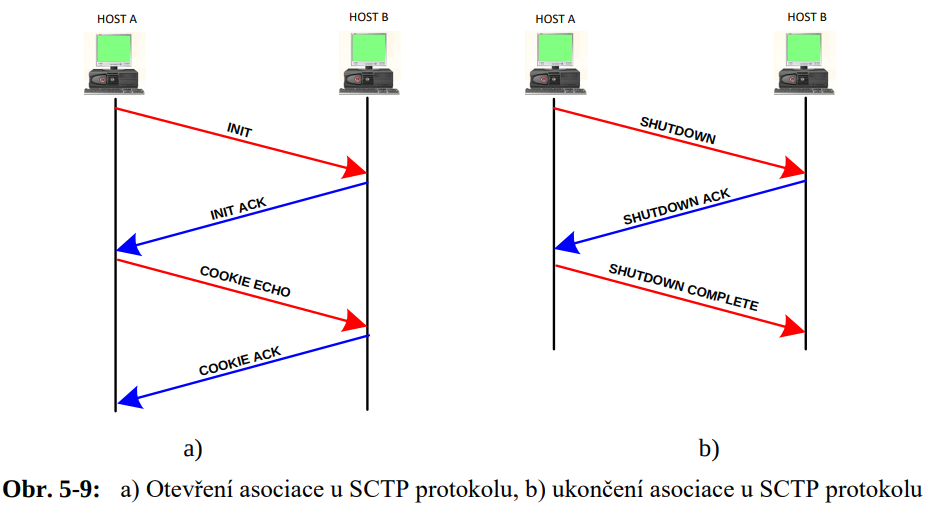
\includegraphics[width=0.6\textwidth]{obrazky/034.png}
\end{figure}

\subsection{QUIC}

Protokol QUIC je podobný TCP a SCTP.
Umožňuje pracovat se spojením které vytváří, udržuje a ukončuje a zároveň během tohoto spojení umí přenášet více nezávislých proudů dat.
QUIC umožňuje řídit datový tok jak na úrovni celého spojení tak na úrovni jednotlivých proudů.
Počet proudů se nemusí ustanovit na začátku spojení.

Dále se snaží snížit čas, který souvisí s režií navazování spojení před skutečným zahájením přenosu dat.
Při navazování spojení spojuje dohromady navazování spojení a ustanovení kryptografického přenosového kanálu.

QUIC se umí vyrovnat se změnou adres na síťové nebo transportní vrstvě během existence spojení.
Nakonec velikost datové části paketu je menší jak u TCP, jelikož využívá protokol UDP a snaží se vyhnout fragmentaci.

\begin{figure}[!h]
    \centering
    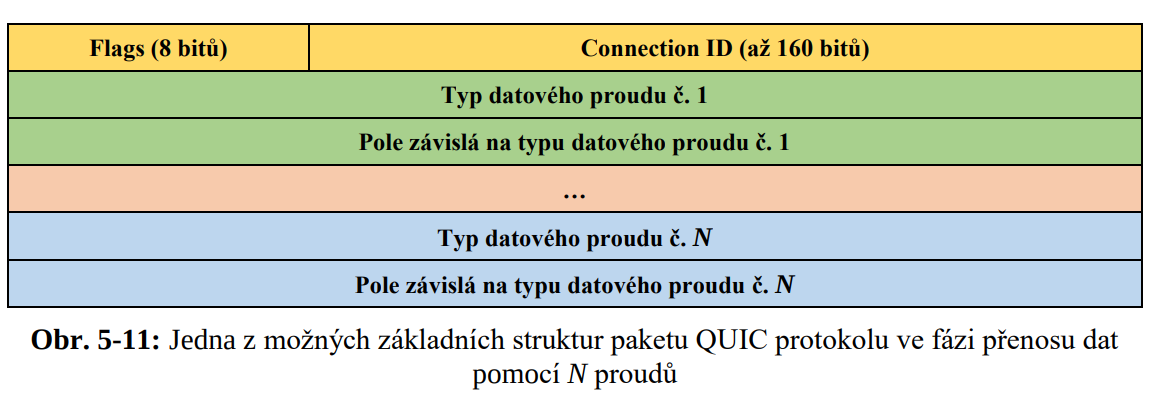
\includegraphics[width=0.5\textwidth]{obrazky/035.png}
\end{figure}


\begin{figure}[!h]
    \centering
    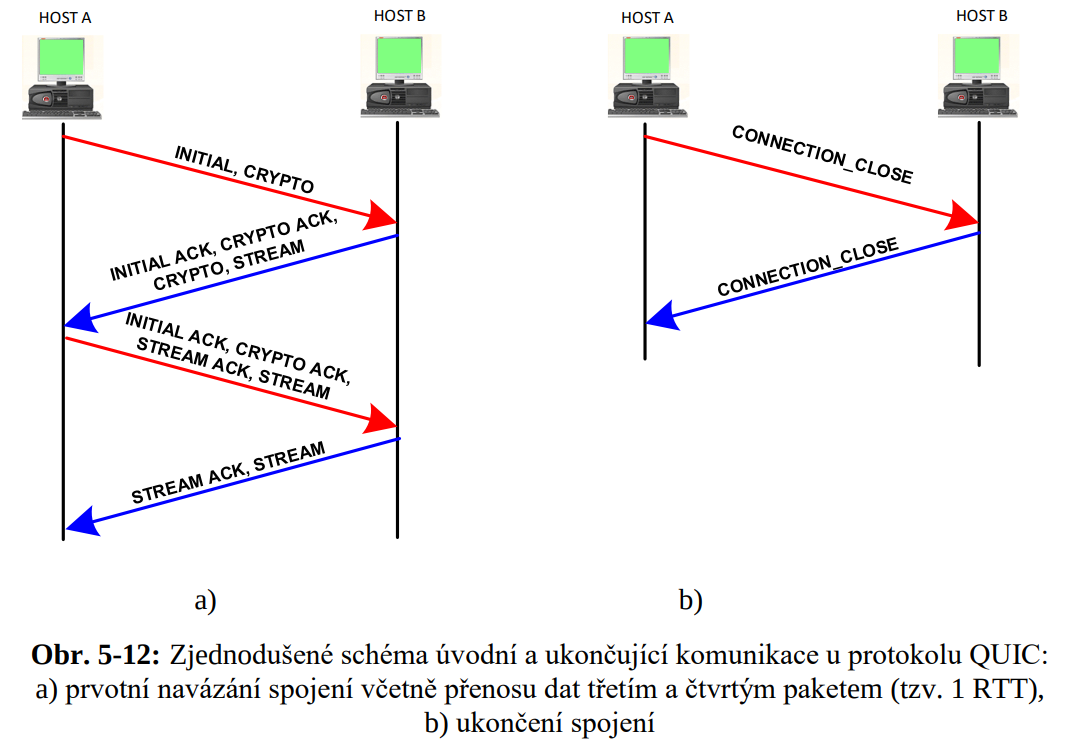
\includegraphics[width=0.55\textwidth]{obrazky/036.png}
\end{figure}


\clearpage
\section{Jmenný systém DNS (Domain Name System): důvody existence, popis fungování protokolu, úloha resolveru, kořenové servery DNS, DNSsec. Protokoly MDNS (Multicast DNS) a LLMNR (Link-Local Multicast Name Resolution).}

\subsection{Důvody existence}
Překládá těžko zapamatovatelné IP adresy na~jednodušeji zapamatovatelná jména v~podobě řetězce znaků.
Pokud by DNS neexistovalo a~tak při~změně IP adresy by si lidé museli znovu zapamatovávat IP adresu.
Při~existenci DNS se přepíše záznam jen na~DNS serveru a~tento problém se nemusí řešit.

\subsection{Popis fungování}

Funguje na~principu klient-server, kdy jedinou IP adresou, kterou musíme znát je adresa DNS serveru.
Ke komunikaci využívá porty UDP 53 a~TCP 53.
Vazba mezi je IP adresou a~doménovým jménem je uložena v~celosvětově distribuované DNS databázi.
Základní jednotkou systému je DNS server (name server, jmenný server, rekurzivní resolver).
DNS servery jsou primární (poskytuje autoritativní odpovědi) a~sekundární (záloha primárního) a~pomocný (pracuje jako vyrovnávací paměť).
Server nejdřív hledá v~pomocném serveru jestli záznam není uložen v~paměti (cache) a~musí mít vlastní DNS server, kterého se může zeptat.

Je vytvářena hierarchie domén, která začíná od kořene a~jde postupně níže.
Prvně se jde od domény nejvyššího řádu k~nižším řádům domény.
Domény nejvyššího řádu se dělí na~generické (.edu, .com) a~národní domény (.cz).
Doménové jméno může mít maximální délku 255 znaků, kdy jeden řád (úroveň) může mít maximálně 63 znaků. Maximální počet řádů může být 127.

Postup dotazu na~fekt.vutbr.cz.
Klient se zeptá lokálního DNS serveru na~IP pro tuto doménu.
Jelikož ten to často neví tak se zeptá kořenových DNS serverů.
Jelikož často kořenový neví, ale ví adresu dalšího DNS serveru pro doménu nejvyššího řádu, tak mu odešle IP na~ten server.
Tak se postupuje stejným způsobem dokud se nenajde server, který danou IP adresu zná.
Tuto IP adresu poté lokální DNS server zašle klientovy\footnote{\url{https://cs.wikipedia.org/wiki/Domain_Name_System\#/media/Soubor:Dns-wikipedia.png}}.

\subsection{Úloha resolveru}

Primární úlohou je překlad doménového jména na IP adresu.
V rámci OS existuje tzv. stup resolver, který zprostředkovává stanicím dotazy na rekurzivní DNS servery.
Než odešle požadavek tak prověří zda překlad není definován staticky nebo není uložen v mezipaměti.
Dotazování na DNS server je často vícenásobné i při jediném překladu.

Postup překladu na mit.edu z domény utko.feec.vutbr.cz.
Uživatel požádá o překlad a jestli překlad nenalezne lokáně resolver se pokusí o dotaz na DNS server.
Jelikož se počítač nachází v doméně utko.feec.vutbr.cz tak resolver prvně vyzkouší jestli mit.edu není lokálním názvem platným v dané doméně.
První požadavek může vypadat jako mit.edu.utko.feec.vutbr.cz.
V tomto případě nic nenalezne a pokusí se o stejný dotaz jenom v doméně vyššího řádu (mit.edu.feec.vutbr.cz).
Tak se to opakuje do doby než je dotaz úspěšný nebo je dotaz neúspěšný i při požití domény druhého řádu (mit.edu.vutbr.cz).
Jelikož byly dotazy neúspěšné resolver požádá DNS server o překlad doménového jména.

\subsection{Kořenové servery DNS}

Kořenové DNS servery obsluhují root doménu.
Tyto servery jsou využívány běžnými rekurzivními DNS servery k přesměrování na jiné doménové servery.
Jejich hlavním úkolem je přesměrování DNs dotazů na jednotlivé DNS servery nejvyšších řádů.

\begin{figure}[!h]
    \centering
    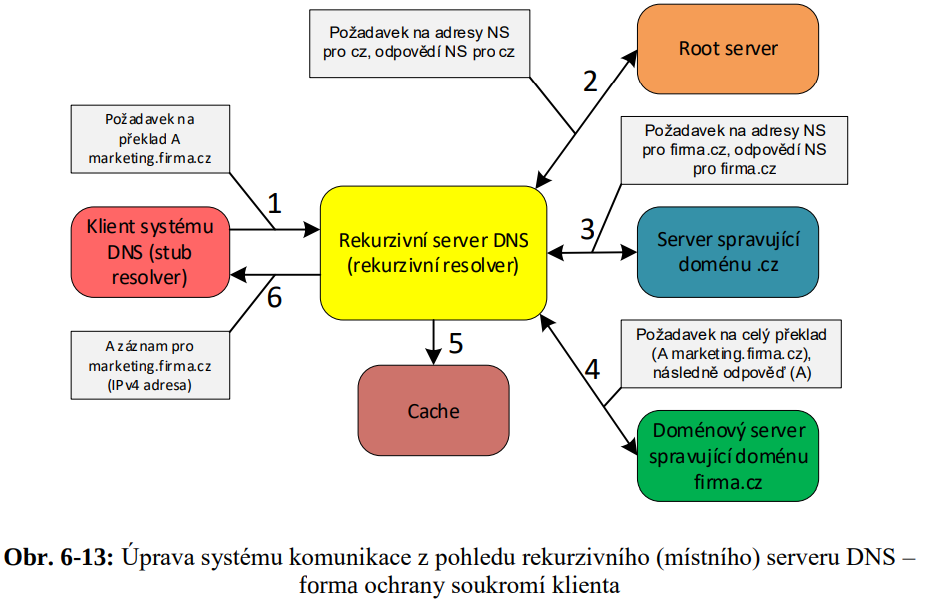
\includegraphics[width=0.7\textwidth]{obrazky/040.png}
\end{figure}

\subsection{DNSsec}

DNSsec poskytuje rozšíření DNS o systém pro ověření autentičnosti obdržených záznamů.
Záznamy jsou digitálně podepisovány, takže pokud důvěřujeme autorovi podpisu, tak můžeme důvěřovat i poskytnuté informaci.
Data nejsou šifrována pouze podepsána.
DNSsec přidává doplňující informace v záznamech jako jsou RRSIG (Resource Record Signature, dig. podpis), DNSKEY (DNS Public Key), DS (Delegation or Designated Signer) a NSEC/NSEC3 sloužící jako záznam zasílaný v odpovědi zpět v případě, že doména je DNS serveru neznámá.





\subsection{MDNS Multicast DNS}

Je doplňující technika k protokolu DNS vyvinutá Applem.
Je součástí skupiny protokolů ZeroConf, což jsou protokoly sloužící k nastavení sítě bez manuálních zásahů administrátorů/uživatelů.

Byl vytvořen aby bylo možné posílat dotazy podobné DNS dotazům pomocí multicastu a bylo by možné aby se okolní stanice byly schopné podílet na odpovědi.
Umožňuje stanicím si zvolit DNS název (nazev.local), který bude využíván pro lokální označování a adresování a umožní tak i bez veřejně platných názvů usnadnění komunikace s využitím lokálních jmenných názvů.
Předpokládá se že doménové jméno končící na .local je platné pouze v lokální síti.

Rozdíly oproti DNS"
\begin{itemize}[noitemsep]
    \item využívá multicast ne unicast
    \item využívá UDP port 5353 ne 53
    \item používá se v přesně definovaných částech jmenného prostoru
    \item pouze UTF-8 kódování
    \item podporuje větší UDP pakety
    \item dovoluje více než jedno jméno v překladu
    \item používá NSEC k signalizaci neexistujícího záznamu
    \item Zkoumá dotazy/odpovědi ostatních stanic, aby zabránil opakování stejných dotazů/odpovědí
\end{itemize}

\subsection{LLMNR Link-Local Multicast Name Resolution}

Multicastové řešení DNS vyvinuto společností Microsoft.
LLMNR zachovává formát paketů a podporuje všechny současné formáty zpráv DNS, typy i třídy.
Využívá port 5355 a využívá jinou cache v rámci OS.
Tvoří doplněk k DNS, jelikož pracuje pouze na lokální lince.

LLMNR dotazy jsou posílány a přijímány na portu 5355 a multicastová adresa uživatelů je 224.0.0.252 a FF02::1:3.
Prlběh je že odesílatel vyšle dotaz na multicast adresu.
Odpovídač na tento dotaz odpoví pouze v případě, že jeho odpověď je autoritativní pro dané doménové jméno.
Odpovídá unicast odpovědí.
Odpověď je po přijetí zpracována a vyhodnocena.


\clearpage
\section{Princip protokolů zálohování výchozí brány. Protokoly HSRP (Hot Standby Router Protocol) a VRRP (Virtual Router Redundancy Protocol).}

\subsection{Podstata}

Pro správné fungování lokálních sítí je důležitá dostupnost výchozí brány.
Na stanicích lze nastavit pouze jednu výchozí bránu a tím pádem problém nastává při jejím výpadku.
Sama stanice nedokáže poznat, že výchozí brána vypadla a mělo by se přepnout na záložní.

Od tohoto existují protokoly pro automatickou konfiguraci výchozí brány.
Základní myšlenou je, že toto provádí sami směrovače, aniž by do toho byly zapojeny stanice.
Protokoly se dělí na dvě skupiny.
První skupinou jsou protokoly které umožňují pouze zálohování dostupnosti výchozí brány (HSRP a VRRRP).
Druhou skupinou jsou protokoly, které umožňují nejen zálohování ale i rozkládání zátěže mezi dostupné výchozí brány (GLBP).

\subsection{HSRP Hot Standby Router Protocol}

HSRP je protokol od společnosti Cisco, který je dostupný na Cisco směrovačích.
Využívá UDP na portu 1985 a k přenosu používá multicast.
HSRP pakety mají nastaven TTL na 1, takže neopustí danou síť.

Funguje tak že více směrovačů má vlastní IP i fyzickou adresu a zároveň tato skupina má jednu virtuální IP adresu a virtuální MAC adresu, která slouží jako výchozí brána.
V každé skupině je zvolen jeden aktivní směrovač, který slouží jako výchozí brána.
Dále bude zvolen záložní směrovač, který čeká na výpadek aktivního směrovače a může okamžitě převzít jeho úlohu.
Pokud je ve skupině víc jak dva směrovače tak ostatní pouze naslouchají komunikaci aktivního a záložního.

Aktivní a záložní směrovač si v pravidelném intervalu vyměňují zprávy a pokud nepřijde zpětná zpráva do určité doby směrovač se považuje za nedostupný.

Protokol také umožňuje že v případě výpadku od aktivního směrovače (směrem ven) je možnost přepnout na záložní směrovač.

\begin{center}
	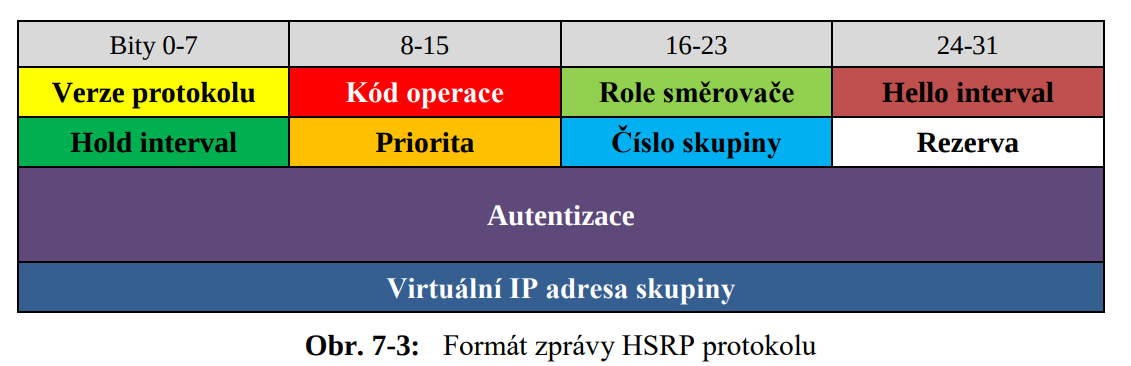
\includegraphics[width=0.53\textwidth]{obrazky/050.png}
\end{center}


\subsection{VRRP Virtual Router Redundancy Protocol}

VRRP poskytuje skoro stejné funkce jako HSRP, ale protokol není omezen pouze na zařízení Cisco.
Tento protokol je vhodné použít pokud jsou v síti směrovače od různých výrobců.

Směrovače které tvoří skupinu si zvolí nositele virtuální IP a MAC adresy.
Tento směrovač se nazývá primární. Ostatní jsou poté ve stavu zálohy a negenerují žádný provoz.

Rozložení zátěže je možné stejně jako u HSRP, že se vytvoří více skupin a tím pádem více výchozích bran.
Takže některé stanice budou mít rozdílné výchozí brány. 

\clearpage
\section{Multicastový přenos dat, adresování, protokoly, směrování multicastu.}

\subsection{Multicast}

Jedná se o přenos jednoho zdroje k skupině příjemců.
Může nastat i případ kdy je zdrojů více.
Od zdroje se vysílá jedna kopie dat, která se po cestě větví na více kopií.

Výhodami multicastu je jeho efektivita oproti unicastu.
Optimalizace zpracování, jelikož přenášeno méně paketů.
Distribuované aplikace, které jsou často bez multicastu nerealizovatelné.

Nevýhodami je chybějící řízení proti zahlcení, vznik duplicitních paketů, doručení paketů v jiném pořadí, nespolehlivost paketů a možnost nežádoucího odposlechu.
Většina těchto nevýhod je způsobena důsledkem využití UDP protokolu, jelikož TCP nemůže být využit kvůli jeho spojovému charakterů. 

\subsection{Adresování}

Adresování pro IPv6 je popsáno v jedné z dalších otázek.

Pro IPv4 má vyhrazen multicast celou třídu D (224.0.0.0 -.239.255.255.255).
Dělí se na tři skupiny.
\begin{itemize}[noitemsep]
    \item Určené pouze pro lokální sítě (224.0.0.0 -- 224.0.0.255)
    \item Pro použití v rámci internetu (224.0.1.0 -- 238.255.255.255)
    \item Pro privátní použití uvnitř domén (239.0.0.0 -- 239.255.255.255) 
\end{itemize}

Pro multicast je vytvořena také MAC adresa (číslo výrobce 01:00:5e), aby se nemusela síť zahlcovat odesíláním na broadcast MAC adresu.
Dále pro ni platí že 25 bit musí být 0.

\subsection{Multicast protokoly}

\subsection{IGMP}

Základní úlohou je umožnit koncovým stanicím připojení do multicastové skupiny.
Slouží ke komunikaci mezi stanicemi a směrovači.
Zprávy jsou přenášeny pouze v lokální síti.
Protokol existuje ve třech verzích.

\subsubsection{IGMPv1}

Tato verze je už zastaralá.
Funguje tak, že směrovač zasílá do lokální sítě periodicky paket membership query na multicast adresu 224.0.0.1.
Stanice poté odpoví na tento dotaz zprávou membership report postupně všem skupinám ke kterým se chtějí připojit.
Pokud se chce odpojit od skupiny tak pouze nereaguje na další membership query.

\subsubsection{IGMPv2}

IGMPv2 přidává možnost zprávy pro okamžité opuštění skupiny.

Jsou 4 typy zprávy:

\begin{itemize}[noitemsep]
    \item Membership query --  stejné jako ve verzi 1
    \item Version 2 Membership Report -- nová verze zprávy pro přihlášení do skupiny
    \item Version 1 Membership Report –- stará verze zprávy přihlášení do skupiny (zpětná kompatibilita)
    \item Leave group -- opuštění skupiny
\end{itemize}

\begin{center}
	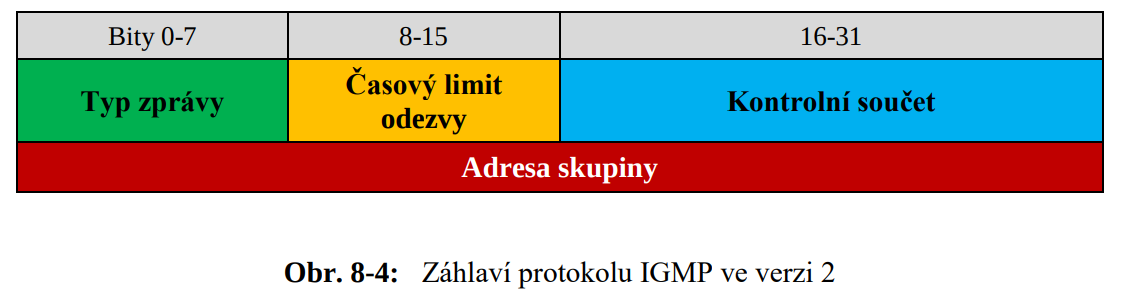
\includegraphics[width=0.7\textwidth]{obrazky/060.png}
\end{center}

\subsubsection{IGMPv3}

Tato verze je navržena také pro co největší zpětnou kompatibilitu.
Novým rozšířením je možnost požadovat nebo filtrovat provoz z individuálních zdrojů v rámci multicastové skupiny.
Stanice si mužou vybírat od koho budou nebo nebudou provoz přijímat.

\begin{center}
	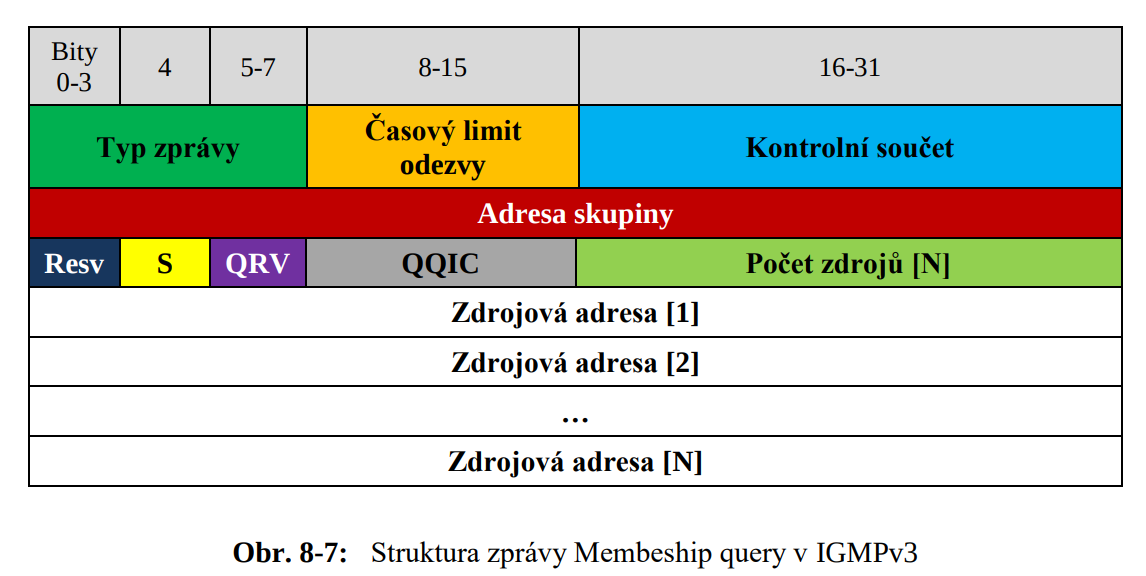
\includegraphics[width=0.7\textwidth]{obrazky/061.png}
\end{center}


\subsection{Směrování multicastu}

Směrování je tvořené nejčastěji ve stromové struktuře pomocí distribučních stromů.
Směrování se v nich provádí pomocí protokolů DVMRP (Distance Vector Multicast Routing Protocol), MOSPF (Multicast Open Shortest Path First), CBT(Core-Based Trees) nebo nejčastěji pomocí PIM (Protocol Independent Multicast).
Každý protokol k hledání co nejefektivnější stormu používá jiné metriky.
Jedinou podmínkou je že ve stromu nesmí existovat smyčka.

Stromy se dělí na dva základní druhy:

\begin{itemize}[noitemsep]
    \item Shortest Path Tree (SPT) -- Snaží se odeslat data nejkratší cestou dál přes další směrovač až k příjemcům.
    Musí existovat pro každý zdroj dat.
    \item Shared Tree -- zde je kořen stromu umístěň uprostřed stromu.
    Zdroje data posílají prvně na tento kořen, a ten je dále pak rozesílá pomocí jediného stromu.
    Tento způsob nemusí být vždy efektivní jelikož může existovat lepší cesta od zdroje k příjemci.
\end{itemize}

\subsubsection{RVP Reverse Path Forwarding}

RPF je mechanizmus, který umožňuje multicastovým směrovačům správně předat pakety skrz distribuční stromy a zároveň se vyvarovat tvoření smyček.
Směrovač u každého paketu sleduje zda směr odkud paket přišel odpovídá cestě ke zdroji dat dané skupiny.
Pokud ano přepošle je přes svá rozhraní které směřují příjemcům.

\subsubsection{PIM Protocol Independent Multicast}

Úkolem PIM je tvorba distribučních stromů, jak sdílených tak nejkratší cesty.
PIM využívá pouze dostupné informace od unicast protokolů.
PIM funguje pouze v autonomních systému, neumí předávat informace mezi nimi.
Základní dva režimy jsou PIM Sparse Mode (PIM-SP) a PIM Dense Mode (PIM-DM). Dalšími varianty jsou Bidirectional PIM a PIM source-specific multicast.

U PIM-SM se předpokládá že multicast nebude v síti převažovat a každá větev se v případě aktivního příjemce musí přidat do stromu a také odebrat.
PIM-SM je založen na distribučním stromu sdíleného typu.
PIM-SM nezaplavuje sítě pakety a proto se zejména nasazuje na rozsáhlých sítích.

U PIM-DM se předpokládá že bude možné směrovat mnoho multicast přenosů a bude se v ní nacházet mnoho příjemců.
Na začátku je síť zaplavena multicast přenosem a ve větvích kde se nenachází příjemce musí dojít k potlačení přenosu.
Pokud se ve větvy nenachází žádný příjemce směrovač musí informovat souseda a přenos do této větve je zastaven.
Směrovač vždy při přijetí kontroluje zda provoz přišel po optimální trase, v případě že ne pakety jsou zahozeny.
PIM-DM slouží primárně pro tvorbu stromů s nejkratší cestou.


\clearpage
\section{IPv6 (Internet Protocol verze 6): vlastnosti protokolu a důvody existence, přechodové mechanizmy, datagram a systém rozšiřujících záhlaví, adresace.}

\subsection{Obecné informace}

IPv6 je nekompatibilní s~IPv4.
Hlavním rozdílem je změna zápisu adres (\texttt{fe80:1a3d::0/64}) a~rozšíření velikosti adresního prostoru z~32 bitů na~128 bitů.
Pro přechodné zajištění kompatibility se využívá technik jako souběh protokolů (SW a~HW podporuje oba dva druhy), tunelování (většinou zapouzdření IPv6 do IPv4 paketu) a~překlad adres (podobné nat jen s~rozdílem že se zaměňují přímo adresy obou verzí, nazývá se to NAT-PT [protocol translator]).

\subsection{Datagram}
\begin{center}
	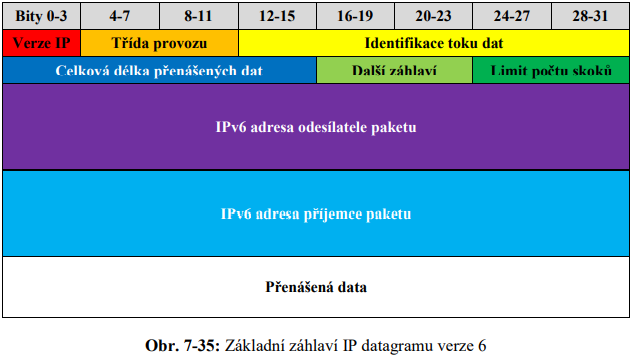
\includegraphics[width=0.6\textwidth]{obrazky/070.png}
\end{center}

Třída provozu nastavuje prioritu paketu, identifikace toku dat umožňuje zjednodušení směrování, celková délka přenášených dat je velikost bez záhlaví, další záhlaví určuje informace o~vnořeném záhlaví.

\subsection{Rozšiřující záhlaví}

Pro každou rozšiřující operaci v IPv6 je zřízena samostatná jednoúčelová hlavička.
V případě kdy je potřeba více operací tak se tyto hlavičky skládají za sebe.Podmínka je aby v každém rozšiřujícím záhlaví byla informace o typu následujícího záhlaví.
Poslední záhlaví obsahuje v tomto poli obsahuje informace o typu přenášených dat.

\subsection{Adresace}

Existují 3 druhy adresování:
\begin{itemize}[noitemsep]
    \item Unicast (individuální) jsou adresy identifikující jednotlivá síťová rozhraní.
    \begin{itemize}[noitemsep]
        \item Globální unikátní (\texttt{2000::/3})
        \item Linkové unikátní (\texttt{FE80::/10})
        \item Lokální smyčka (\texttt{::1/128})
        \item Nespecifikovaná adresa (\texttt{::/128})
        \item lokální unikátní (\texttt{FC00::/7})
        \item IPv4 kompatibilní (\texttt{::/80})
    \end{itemize}
    \item Multicast (skupinové) pro skupiny a~pakety jsou doručeny všem ve~skupině. Patří sem i~broadcast adresy.
    \begin{itemize}[noitemsep]
        \item Přiřazená adresa (\texttt{FF00::/8})
        \item Vyzývaný uzel (\texttt{FF02::1:ff00:0/104})
    \end{itemize}
    \item Anycast (výběrové) také skupina ale paket je do doručen pouze jedinému členovy (nejčastěji nejbližší).
\end{itemize}

\begin{center}
	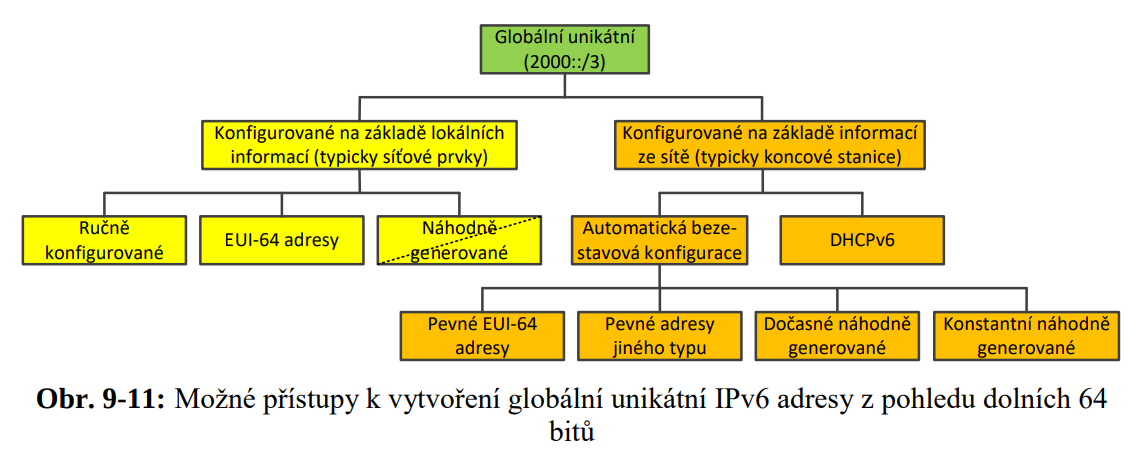
\includegraphics[width=0.9\textwidth]{obrazky/071.png}
\end{center}


\clearpage
\section{IPv6 (Internet Protocol verze 6): funkce ICMPv6 protokolu, popis automatické konfigurace v IPv6 síti, fungování multicastu v IPv6.}

\subsection{ICMPv6}

ICMPv6 je servisním protokolem.
Nemá za úkol přenášet žádná data.
Pokud není implementován je IPv6 nefunkční.
Slouží k ohlašování chybových stavů, dostupnosti zařízení a výměně určitých provozních informací.
V rámci IPv6 slouží k Neighbor Discovery.

Formát zprávy se skládá z typu (určuje druh zprávy), kódu (specifikuje blíže typ), kontrolního součtu a těla zprávy (záleží na typu).

Vybrané skupiny s čísly typu zprávu:
\begin{itemize}[noitemsep]
    \item Chyby -- čísla 1 (nedosažitelný), 2, 3 (TTL vypršelo), 4
    \item Echo -- 128 (dotaz), 129 (odpověď)
    \item Neighbor Discovery -- 133, 134, 135, 136, 137
    \item Informace o uzlu -- 139 (dotaz na informace), 140 (odpověď)
    \item Inverzní objevování sousedů -- 141 (výzva), 142 (ohlášení)
\end{itemize}

\subsection{Neighbor Discovery}

Neighbor Discovery (ND) se využívá pouze v rámci jedné sítě.
Hlavním cílem ND je překlad IP adres na fyzické, k čemu je v IPv4 využíván protokol ARP.
Dále muže sloužit k:
\begin{itemize}[noitemsep]
    \item Aktualizace neplatných položek a zjišťování změn ve fyzických adresách
    \item Hledání směrovačů
    \item Přesměrování
    \item Zjišťování prefixů, parametrů sítě a dalších údajů pro automatickou konfiguraci adresy
    \item Ověření dosažitelnosti sousedů
    \item Detekce duplicitních adres
\end{itemize}

ND využívá ke všem operacím ICMPv6 zprávy.
Postup ND je podobný jako v případě ARP avšak jsou změny jsou provedeny v přejmenování zpráv (výzva sousedovi -- neighbor solicitation, ohlášení souseda -- neighbor advertisement).
Pro zasílání zpráv je využívána multicast skupina s prefixem ff02:0:0:0:0:1:ff00::/104.
Posledních 24 bitů adresy se vytvoří tak že z hledané adresy se odebere nejnižších 24 bitů.
Tato adresa se poté nazývá vyzývavý uzel.
Stanice musí při startu síťového uzlu vstoupit do všech skupin odpovídajících adresám vyzývaného uzlu.
Takže zprávu výzva sousedovi nedostane každý v síti, ale jen stanice které mají posledních 24 bitů shodných.

K ověřování platnosti adresy se využívá detekce dosažitelnosti souseda.
Uzel v IPv6 aktivně monitoruje stav sousedů.
K potvrzení dostupnosti lze využít, že právě teď probíhá komunikace mezi nimi nebo stanice zašle výzvu sousedovi, aby ověřila jeho dostupnost.

ND má taky verzi SEND (SEcure Neighbor Discovery), kdy se využívá RSA k digitálnímu podpisu.
Ke komunikaci využívá ICMPv6 typů 148 (žádost o certifikační cestu) a 149 (ohlášení certifikační cesty).

\subsection{Automatická bezstavová konfigurace}

Základním principem bezstavové adresní konfigurace (SLAAC) je, že směrovač do sítě vysílá opakovaně potřebné informace pomocí ICMPv6 zprávy typy 134 (ohlášení směrovače/router advertisment).
Stanice může o tyto informace požádat pomocí zprávy typu 133 (výzva směrovači).
Stanice na základě přijatý informací stanoví vlastní IP adresu.
Informace umožní stanicím v síti vědět, kde se nacházejí, jak se mají chovat a kdo je implicitní směrovač.


Při odesílání paketu se stanice nejdřív podívá do lokální cache, zda nemá už záznam o komunikaci.
Pokud ne zjišťuje na základě seznamu prefixů zda je stanice lokální nebo vzdálená.
Pokud je lokální tak se aplikuje ND.
Pokud není je zvolen vhodný implicitní směrovač a na něj odeslat paket.
Pokud zvolený směrovač není vhodný tak zašle ICMPv6 zprávu typu 137 (přesměrování), obsahujicí kam by se měl paket odeslat.

\subsection{DHCPv6}

Podobný obyčejnému DHCP, jen se nevyužívají broadcast zprávy, ale multicast zprávy.
Stále zde zůstává klient, server a zprostředkovatel (relay, předává zprávy mezi klientem a servem).
Identifikace stanic je postavena na DUID (DHCP Unique IDentifier) a měl by být neměnný pro všechny klienty a servery.
DUID je pro celé zařízení, ne jednotlivá síťová rozhraní.

Typy vytvoření DUID:

\begin{itemize}[noitemsep]
    \item Stanovení výrobcem
    \item Kombinace fyzické adresy s časovým údajem
    \item Pouze fyzická adresa, avšak DUID by měl být využíván pro celou stanici
\end{itemize}

Pro rozlišeni jednotlivých rozhraní se používá IA (Identity Association). IA je jenom shluk konfiguračních informací, Tento shluk má jednoznačný identifikátor IAID.

\subsubsection{Stavové DHCPv6}

Představuje plnou verzi protokolu a odpovídá DHCPv4.
Jsou zde tři odlišnosti.
Prvním je že u IPv4 je DHCPv4 paket zpravidla prvním paketem stanice odeslaným do sítě, ale i IPv6 je toto volitelný krok v závislosti co se stanice dozví od směrovače.
Druhým je že jednotlivé zprávy se jmenují jinak.
Třetím je že se pro přenos nepoužívá broadcast ale multicast.

\subsubsection{Bezstavové DHCPv6}

Bezstavová DHCPv6 je zjednodušená verze DHCPv6.
Zprávy mají stejný formát ale pužívají se pouze dva typy zpráv (žádost o informace a odpověď).
Používá se hlavně pokud si stanice umí nakonfigurovat samy IPv6 adresu ale potřebují informace o DNS.

\subsection{MLD Multicast Listener Discovery}

MLD není samostatný protokol ale podmnožina ICMPv6.
Pakety MLD mají počet skoků nastaven maximálně na 1.
V případě že je odeílatel směrovač, jako IPv6 adresa odesílatele je využita lokální linková adresa daného rozhraní (local-link).
Adresátem je pak IPv6 adresa multicastové skupiny.
MLD paket musí obsahovat rozšiřující IP záhlaví označované jako volby pro všechny (hop-by ho option).

Existují 3 ICMPv6 typy zpráv (130 -- dotaz na členstvý ve skupině, 131 -- ohlášení členství ve skupině, 132 -- ukončení člensví ve skupině).


\subsubsection{MLDv1}

MLDv1 nebsahuje mechanizmy pro práci s konkrétními odesílateli takže je dostatečné když směrovač pracuje se skupinami (zda pro skupinu existuje nějaký příjemce).
Na základě tohoto se pak vytvářejí distribuční stromy.
Směrovač je povinný přijímat pakety adresované libovolné multicastové skupině.

Vstup do skupiny probíhá odesláním zprávy na multicast adresu skupiny (typ zprávy report).
Vystoupení skupiny probíhá odesláním zprávy typu done na všechny směrovače na dané lince (ne na danou multicast skupinu).
Obecný dotaz na členství probíhá odesláním zprávy query směrovačem na všechny uzly na lince.
Každá stanice si nastaví pro všechny skupiny kterých je členem samostatný časovač.
Po vypršení časovače pošle na adresu skupiny ohlášení svého členství.

\subsubsection{MLDv2}

Výhodou MLDv2 je možnost filtrovat příjem multicastu na základě zdroje.
Lze také požadovat příjem pouze od vybraných zdrojů (INCLUDE), nebo přijímat multicast od všech kromě specifikovaných (EXCLUDE).

Byla odstraněna zpráva pro odchod ze skupiny (done).
Tato zpráva byla nahrazena zprávou typu 143 report (změna příjmu skupin).
Tato zpráva umožňuje využití pro přihlašování i odhlašování.

Pro zjednodušení v praxi byla vytvořena varianta Lightweight MLDv2, která nemá všechny funkce ale zjednodušuje celý mechanismus.


\clearpage
\section{Autonomní systémy. Protokoly IGP (Interior Gateway Protocol) a EGP (Exterior Gateway Protocol). Základní charakteristika protokolu BGP (Border Gateway Protocol). Multihoming, peering a tranzit.}

\subsection{Autonomní systémy}

Autonomní systém (AS) představuje souhrn sítí pod společnou správou, kde se používá společná směrovací strategie.
Autonomní systém je dělen na menší oblasti.
Každý AS musí mít přiřazené unikátní 16bitové číslo (nově 32bitové).
Toto číslo se přiděluje centrálně v rámci celé světové sítě.

\subsection{IGP Interior Gateway Protocol}

IGP slouží jako označení pro směrovací protokoly uvnitř autonomního systému.
Takže sem spadá RIPv2, EIGRP, OSPF, IS-IS

\subsection{EGP (Exterior Gateway Protocol}

Protokol EGP slouží pro vzájemnou komunikaci mezi AS.
Vychází z představy že v rámci každého AS je alespoň jedna brána pověřena předáváním směrovacích informací mimo AS (ven).
Tuto bránu vybírá správce AS a je označena jako externí brána.
Tato brána pak komunikuje s ostatními externími branami jiných AS.

Protokol umožňuje dohodu mezi dvěma AS jestli si budou směrovací informace vůbec vyměňovat.
Dále je umožněno, aby AS pravidelně testoval dostupnost ostatních AS.
Hlavní úkol je avšak pravidelný přenos směrovacích údajů a informací o průběžných změnách mezi AS.

\subsection{BGP Border Gateway Protocol}

Protokol BGP je náhrada za protokol EGP.
Hlavním cílem BGP je dosažení flexibility a možnosti snadné volby propojení a výměny směrovacích záznamů mezi AS.
Informace se vyměňují mezi sousedy a spojení mezi těmito směrovači musí být nakonfigurováno ručně.
BGP využívá TCP port 179.

AS svým sousedním AS pomocí BGP sděluje k jakým IP sítím je schopen doručit pakety.
Okolní AS se rozhodnou zda použijí konkrétní AS pro směrování k dané síti.

\begin{figure}[!h]
    \centering
    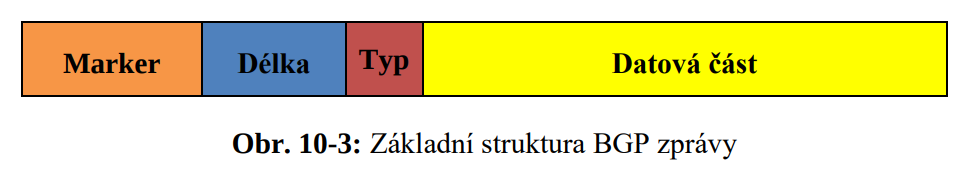
\includegraphics[width=0.7\textwidth]{obrazky/091.png}
\end{figure}

\begin{itemize}[noitemsep]
    \item Marker 16B -- pouze z důvodu kompatibility, vyplněno binárními jedničkami
    \item Délka 2B -- délka zprávy, min 19 a max 4096
    \item Typ 1B -- kód zprávy, 4 typy
    \begin{itemize}[noitemsep]
        \item Open -- úvodní zpráva
        \item Update -- aktualizace tabulek
        \item Notification -- zrušení spojení při chybě/mimořádné situaci
        \item KeepAlive -- pravidelné opakování
    \end{itemize}
    \item Datová část -- nepovinná část délky
\end{itemize}



BGP lze využít i pro směrování uvnitř AS.
V takovém případě se označuje jako iBGP (internal BGP).
Nejčastěji se využívá při přenosu směrovacích informací mezi dvěma nebo více hraničními branami v rámci jednoho AS.
Tímto se docílí správného rozhodnutí jaký směr pro směrování zvolit, pokud je více možností.
V tomto případě je nutné aby hraniční směrovače byly propojené každý s každým.

V případě komunikace mezi AS se někdy využívá název eBGP (external BGP).

\begin{figure}[!h]
    \centering
    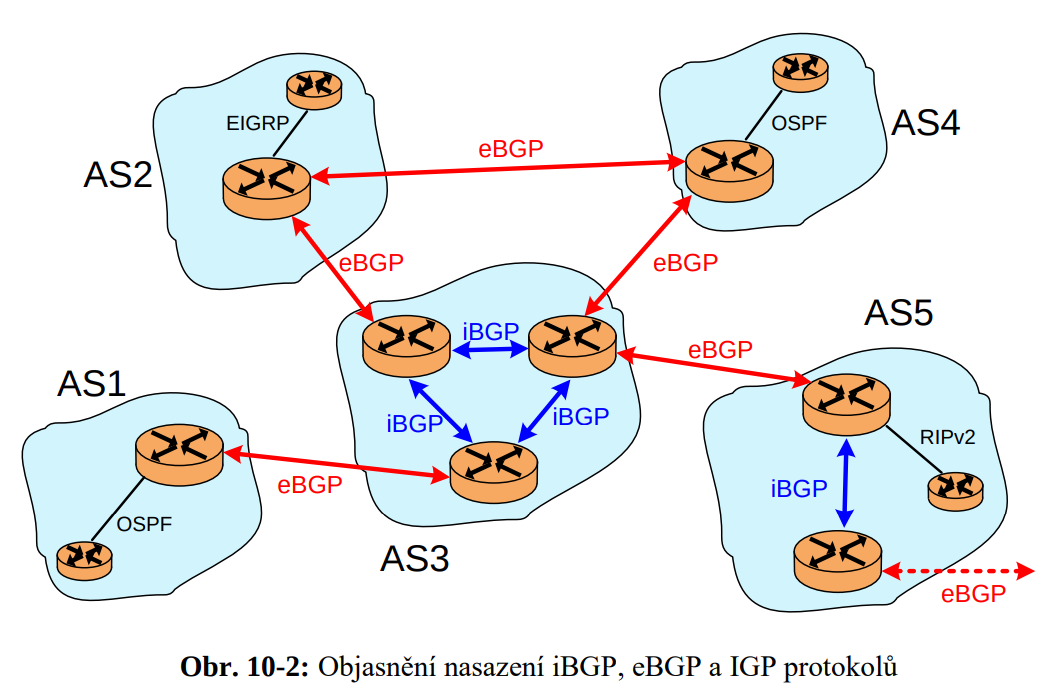
\includegraphics[width=0.7\textwidth]{obrazky/090.png}
\end{figure}


\subsection{Multihoming}

Multihoming je technika zajištující zvýšení spolehlivosti Internetové konektivity pro konkrétní síť.
Snaží se eliminovat ztrátu konektivity, ke které by mohlo dojít prostřednictvím chyby jediného bodu.
Existuje několik variant.

\begin{itemize}[noitemsep]
        \item Jedna fyzická linka, více IP adres -- úvodní zpráva
        \item Více fyzických linek, jedna IP adresa na každou z nich -- aktualizace tabulek
        \item Notification -- zrušení spojení při chybě/mimořádné situaci
        \item KeepAlive -- pravidelné opakování
\end{itemize}

\subsubsection{Jedna fyzická linka, více IP adres}

Tato varianta je nejméně bezpečná.
Host má k dispozici více IP adres, od různých poskytovatelů ale je připojen pomocí jedné fyzické linky.
Při výpadku poskytovatele se přejde na druhého.
Při výpadku linky nebude konektivita.

\subsubsection{}
\begin{itemize}[noitemsep]
        \item Každý ISP předává do našeho AS pouze informaci o default route do svého AS a tato informace je předávána směrovačům našeho AS.
        Ven se předávají kompletní informace o kompletních existujících sítích.
        \item Každý ISP předává do našeho AS default route a specifické směrovací informace (nekompletní), nejčastěji o dostupnosti sítí ve svém AS.
        V tomto případě lze všechny informace předat interním směrovačům v našem AS pomocí transformace informací do některého z IGP protokolu.
        Nebo muže být využito BGP/iBGP.
        \item Každý ISP předává všechny směrovací informace, které má k dispozici.
        Všechny směrovače pracují s BGP.
        V této situaci je vhodné použití filtrování rout aby zákazník nebyl tranzitivním mezi svými poskytovateli.
\end{itemize}

\subsubsection{Více fyzických linek, jedna IP adresa na každou z nich}

Při výpadku jednoho poskytovatele nebo fyzické linky zůstává další linka a konektivita je ztracena pouze na krátké období přepnutí na jinou linku.

\subsubsection{Více fyzických linek, jedna IP adresa }

Považováno za čistý multihoming.
Koncová síť používá pouze 1 IP adresu, která je používána na jedné z linek.
Pokud tato linka přestane fungovat přepne se na jinou linku.

\subsubsection{Více fyzických linek, více IP adres}

Dochází k současnému využití služeb několika poskytovatelů.
Díky tomuto dojde ke zvýšení spolehlivosti a kapacity celé konektivity.
Může se zde využívat load balancing, kdy se zátěž rozděluje rovnoměrně mezi jednotlivé linky.

\subsection{Peering}

Peering představuje pojem pro přímé propojení administrativně samostatných sítí.
Nejčastěji se jedná o propojení nezávislých AS.
Příkladem může být ISP.
Hlavní důvod je umožnit výměnu dat mezi uživateli propojených sítí.

\subsubsection{Privátní peering}

Jedná se o přímé propojení dvou sítí navzájem.
Tato linka je vyhrazena pouze pro jedno konkrétní spojení a nesdílí se s dalšími stranami.
Význam má v případě velkého datového provozu, jelikož může být velmi rychlé.
Není však možné takto propojovat každý AS navzájem, jelikož by byl velký počet spojení.

\subsubsection{Veřejný peering}

Propojení více než dvou stran v jednom bodě.
Tyto body jsou označovány jako exchanges points.
K těmto bodům jsou připojeny až stovky AS, které jsou vzájemně propojené.
Nelze dosáhnout maximální rychlosti mezi linkami.

\subsection{Tranzit}

Druhým způsobem propojení AS je tranzit.
Spočívá v tom, že všechny koncové AS jsou připojeny na páteřní síť, která zajišťuje tranzit datového provozu.
Páteřní síť je také AS.

Tranzit se skládá ze dvou služeb.
První je že poskytovatel oznamuje připojenému AS informace o routách k sítím svých zákazníků, čímž umožní příchozí provoz z celého internetu.
Druhou službou je informování sítí zákazníků o routách do internetu (např. výchozí brána).
Toto umožňuje zákazníkovy vytvářet odchozí provoz.

Rozdíl s peeringem je, že přes peeringové spojení dvou ISP prochází pouze přenos mezi zákazníky těchto dvou sítí.
Na rozdíl od tranzitu, kdy přes toto spojení může procházet i přenos směřující z/do jiného AS.


\clearpage
\section{Teorie konečných automatů a její použití v oblasti komunikačních protokolů, způsoby grafické reprezentace.}

Každý systém lze popsat pomocí stavů vstupních veličin X, kde X se mění v závislosti na čase a pomocí výstupních veličin Y, jejich hodnoty jsou zpravidla závislé na vstupních veličinách.
Zároveň se dá předpokládat že v systému existují vnitřní stavy označované jako Q.
Každá veličina X, Y a Q může být v systému 1-n, kde je konečné diskrétní číslo.
Pro každou veličinu může být konečné číslo jiné.
Existují dva typy systémů (Kombinační sítě a sekvenční sítě).

\subsection{Kombinační sítě}

Kombinační sítě jsou charakterizovány jednoznačným přiřazením výstupní kombinace na každou vstupní kombinaci.
Tyto systémy nemají žádné vnitřní stavy Q.
Vnitřní stavy Q jsou nahrazeny funkcí f, která jednoznačně převádí vstupní vektor X na výstupní vektor Y.

\subsection{Sekvenční sítě}

Sekvenční sítě mají nějak zakomponovanou vnitřní paměť, která jim umožňuje udržovat si informaci o vnitřním stavu Q.
Hodnoty výstupního vektoru Y nezávisí pouze na vstupním vektoru X ale také na vnitřním stavu Q.
Systém se skládá ze vstupních vektorů X, výstupních vektorů Y, vnitřních stavů Q (jsou dané pamětí obsahující informace o předešlých stavech) a operací.
V rámci operace si pro každé $n\ge0$ síť spočítá pomocí vstupního vektoru X v daném kroku a aktuálního vnitřního stavu Q nový vnitřní stav Q.

Algoritmus sekvenční sítě musí mít vlastnosti:
\begin{itemize}[noitemsep]
    \item Determinizmus -- poskytované řešení musí být jednoznačné
    \item Hromadnost -- musí poskytovat možnost řešení skupiny úloh
    \item Konečnost -- počet vnitřních stavů je omezen
\end{itemize}

\subsection{Tabulky přechodů a výstupů}
\textbf{Tabulka přechodů} bude obsahovat výchozí stav $Q_n$ a následný stav $Q_{n+1}$, který byl vyvolán vstupem~X.

\textbf{Tabulka výstupů}  obsahuje výchozí stav Q a odezvu na výstup Y vyvolanou jedním z možných vstup~X.

\subsection{Grafická reprezentace automatů}

\subsubsection{Mealyho automat}

U Mealyho automatu platí že každý uzel určuje jeden stav Q.
Existuje tolik uzlů kolik existuje stavů.
Pro pár stavů Q existuje nula, jeden nebo více přechodů zapsaných pomocí orientovaných křivek.
Nad křivkou je označeno jaký vstup X a jaký výstup Y je očekáván.

\subsection{Mooreho automat}

U Moorova automatu platí že každý uzel je označen stavem Q a odpovídajícím výstupem Y.
Nad spojovací křivkou je v tom případě označeno pouze X.
Výhodou Moorova automatu je snadná čitelnost popisu chování dané sítě.


\subsection{Příklad viz skripta}

Mějme konečný automat, který realizuje triviální funkci detektoru binární (sériové)
sekvence 011.
Detektor má jeden vstup a jeden výstup, přičemž množina všech vstupů je X = {1, 0}, (X1 = 1, X2 = 0) a množina všech možných výstupů Y = {0, 1}, kde „Y1 = 0“ znamená, že hledaná posloupnost dosud nebyla detekována, hodnota „Y2 = 1“ opak.
Automat má definovány celkem čtyři vnitřní stavy – Q1, Q2, Q3 a Q4, přičemž Q1 je výchozím stavem, Q4 konečným stavem.
Automat svou činnost zdárnou detekcí hledané posloupnosti 011 končí a na libovolný vstup už žádným způsobem nereaguje a zůstává v konečném stavu Q4.

\subsubsection{Tabulka výstupů}

\begin{table}[ht]
    \begin{tabular}{ccc}
    \hline
                 & \multicolumn{2}{c}{Vstup} \\
    Výchozí stav & $X_1$       & $X_2$       \\\hline
    $Q_1$        & $Y_1$       & $Y_1$       \\
    $Q_2$        & $Y_1$       & $Y_1$       \\
    $Q_3$        & $Y_2$       & $Y_1$       \\
    $Q_4$        & $Y_2$       & $Y_2$       \\\hline
    \end{tabular}
\end{table}

\subsubsection{Tabulka přechodů}

\begin{table}[ht]
    \begin{tabular}{ccc}
    \hline
                 & \multicolumn{2}{c}{Vstup} \\
    Výchozí stav & $X_1$       & $X_2$       \\\hline
    $Q_1$        & $Q_1$       & $Q_2$       \\
    $Q_2$        & $Q_3$       & $Q_2$       \\
    $Q_3$        & $Q_4$       & $Q_2$       \\
    $Q_4$        & $Q_4$       & $Q_4$       \\\hline
    \end{tabular}
\end{table}

\subsubsection{Mealyho a Mooreho automat}

\begin{figure}[!h]
    \centering
    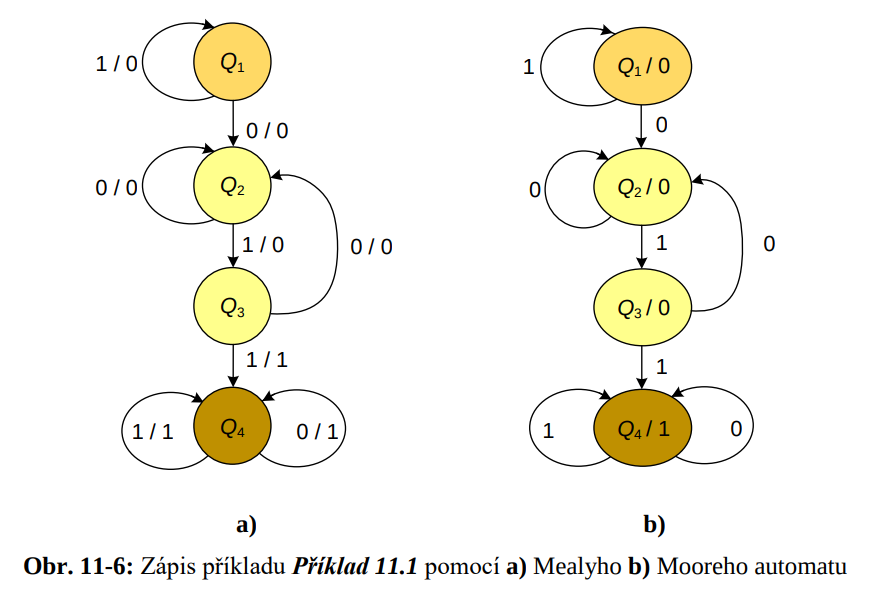
\includegraphics[width=0.7\textwidth]{obrazky/100.png}
\end{figure}

